\documentclass{book}

\usepackage{graphicx}
\usepackage{xkeyval}
\usepackage{multirow}
%\usepackage{bm} %% bold face math symbols
%\usepackage{listings}
\usepackage{../macros/mytikz}
%\usepackage{multicol}
\usepackage{stmaryrd}%\newcommand{\contra}{\lightning}
%\usepackage{rotating} \newcommand{\sw}[1]{\begin{sideways}#1\end{sideways}}

%\usepackage{../macros/algorithm}
%\usepackage{ded}

\usepackage{../mylecturenotes}

\title{Lectures Notes on Knowledge Representation and Processing}
\author{Florian Rabe (for a course given with Michael Kohlhase)}
\date{2020}

\begin{document}
\maketitle


\bigskip

These notes were originally prepared for my CS course at University Erlangen-Nuremberg (FAU) given with Michael Kohlhase in Summer 2020.
They are directed at 3rd semester CS undergraduates and master students but should be intelligible even for earlier students and could be interesting also for PhD students and for students from adjacent majors.
The course is recommended both as a first course in the specialization area Artificial Intelligence as well as a one-off overview on on knowledge representation.

The course was developed in Summer 2020 from scratch and materials were built along the way.
It integrated current directions and recent results in research on knowledge representation pulling together materials in an entirely new and original way.

\tableofcontents

\newpage

% % % % % % % % % % % % % % % % % % % %
\part{Introduction}\label{sec:wuv:intro}

\chapter{Meta-Remarks}
  \begin{center}
\textbf{Important stuff that you should read carefully!}
\end{center}

\paragraph{State of these notes}
I constantly work on my lecture notes.
Therefore, keep in mind that:
\begin{compactitem}
\item I am developing these notes in parallel with the lecture --- they can grow or change throughout the semester.
\item These notes are neither a subset nor a superset of the material discussed in the lecture. On the one handle, they may contain more details than mentioned in the lectures. On the other hand, important material such as background, diagrams, and examples may be part of the lecture but not mentioned in these notes.
\item Unless mentioned otherwise, all material in these notes is exam-relevant (in addition to all material discussed in the lectures).
\end{compactitem}
\medskip

\paragraph{Collaboration on these notes}
I am writing these notes using LaTeX and storing them in a git repository on GitHub at \url{https://github.com/florian-rabe/Teaching}.
As an experiment in teaching, I am inviting all of you to collaborate on these lecture notes with me.
This would require familiarity with LaTeX as well as Git and GitHub --- that is not part of this lecture, but it is an essential skill for you.
Ask in the lecture if you have difficulty figuring it out on your own.
\medskip

By forking and by submitting pull requests for this repository, you can suggest changes to these notes.
For example, you are encouraged to:
\begin{compactitem}
\item Fix typos and other errors.
\item Add examples and diagrams that I develop on the board during lectures.
\item Add solutions for the homeworks if I did not provide any (of course, I will only integrate solutions after the deadline).
\item Add additional examples, exercises, or explanations that you came up or found in other sources.
 If you use material from other sources (e.g., by copying an diagram from some website), make sure that you have the license to use it and that you acknowledge sources appropriately!
\end{compactitem}
I will review and approve or reject the changes.
If you make substantial contributions, I will list you as a contributor (i.e., something you can put in your CV).
\medskip

Any improvement you make will not only help your fellow students, it will also increase your own understanding of the material.
%Therefore, I can give you up to $10\%$ bonus credit for such contributions.
Make sure your git commits carry a user name that I can connect to you.)

\paragraph{Other Advice}
I maintain a list of useful advice for students at \url{https://github.com/florian-rabe/Teaching/blob/master/general/advice_for_students.pdf}.
It is mostly targeted at older students who work in individual projects with me (e.g., students who work on their BSc thesis).
But much of it is useful for you already now or will become useful soon.
So have a look.

\chapter{Fundamental Concepts}\label{sec:wuv:concepts}
  \section{Abbreviations}

\begin{center}
\begin{tabular}{lll}
knowledge representation and processing & KRP & the general area of this course \\
knowledge representation language & KRL & a languages used in KRP \\
knowledge representation tool & KRT & a tool implementing a KPL and processing algorithms for it
\end{tabular}
\end{center}

\section{Motivation}

\subsection{Knowledge}

Human knowledge pervades all sciences including computer science, mathematics, natural sciences and engineering.
That is not surprising: ``science'' is derived from the Latin word ``scire'' meaning ``to know''.
Similarly, philosophy, from which all sciences derive, is named after the Greek words ``philo'' meaning loving and ``sophia'' meaning wisdom, and the for common ending ``-logy'' is derived from Greek ``logos'' meaning word (i.e., a representation of knowledge).

In regards to knowledge, computer science is special in two ways:
Firstly, many branches of computer science need to understand KRP as a prerequisite for teaching computers to do knowledge-based tasks.
In some sense, KRP is the foundation and ultimate goal of all artificial intelligence.%
\footnote{Indeed, a major problem with the currently very successful machine learning-based AI technology is that it remains unclear when and how it does KRP. That can be dangerous because it leads to AI systems recommending decisions without being able to explain why that decision should be trusted.}
Secondly, modern information technology enables all sciences to apply computer-based KRP in order to vastly expand on the domain-specific tasks that can be automated.
Currently all sciences are becoming more and more computerized, but most non-CS scientists (and many computer scientists for that matter) lack a systematic education and understanding of IT-KRP.
That often leads to bad solutions when domain experts cannot see which KRP solutions are applicable or how to apply them.

\subsection{Representation and Processing}

It is no coincidence that this course uses the phrase ``Representation and Processing''.
In fact, this is an instance of a universal duality.
Consider the following table of analogous concept pairs, which could be extended with many more examples:

\begin{center}
\begin{tabular}{l|l}
Representation & Processing \\
\hline
Static & Dynamic \\
Situation & Change \\
Be & Become \\
Data Structures & Algorithms \\
Set & Function \\
State & Transition \\
Space & Time
\end{tabular}
\end{center}

Again and again, we distinguish a static concept that describes/represents what is a situation/state is and a dynamic concept that describes how it changes.
If that change is a computer doing something with or acting on that representation, we speak of ``processing''.

It is particular illuminating to contrast KRP to the standard CS course on Data Structures and Algorithms (DA).%
\footnote{The course is typically called ``Algorithms and Data Structures'', but that is arguably awkward because algorithms can exist if there are data structure to work with. Compare my notes on that course in this repository, where I emphasize data structures much more than is commonly done in that course.}
Generally speaking, DA teaches the methods, and KRP teaches how to apply them.
Data structures are a critical prerequisite for representing knowledge.
But data structures alone do not capture what the data means (i.e., the knowledge) or if a particular representation makes any sense.
Similarly, algorithms are the critical prerequisite for processing knowledge.
But while algorithms can be systematically analyzed for efficiency, it is much harder to analyze if an algorithm processes knowledge correctly.
The latter requires understanding what the input and output data means.

Capturing knowledge in computers is much harder than developing data structures and algorithms.
It is ultimately the same challenge as figuring out if a computer system is working correctly --- a problem that is well-known to be undecidable in general and very difficult in each individual case.

%%%%%%%%%%%%%%%%%%%%%%%%%%%%%%%%%%%%%%%%%%%%%%%%%%%%%%%%%%%%%%%
\section{Components of Knowledge}

\subsection{Syntax and Semantics, Data and Knowledge}

Four concepts are of particular relevance to understanding knowledge.
They form a $2\times 2$-quadruple of concepts:

\begin{center}
\begin{tabular}{l|l}
Syntax & Data \\
\hline
Semantics & Knowledge
\end{tabular}
\end{center}

All four concepts are primitive, i.e., they cannot be defined in simpler terms.
All sciences have few carefully-chosen primitive on which everything builds.
This is done most systematically in mathematics (where primitives include set or function).
While mathematical primitives as well as some primitives in physics or CS are specified formally, the above four concepts can only be described informally, ultimately appealing to pre-existing human understanding.
Moreover, this description is not standardized --- different courses may use very different descriptions even they ultimately try to capture the same elusive ideas.

\textbf{Data} (in the narrow sense of computer science) is any object that can be stored in a computer, typically combined with the ability to input/output, transfer, and change the object.
This includes bits, strings, numbers, files, etc.

Data by itself is useless because we would have no idea what to do with it.
For example, the object $O=((49.5739143, 11.0264941), "2020-04-21T16:15:00CEST")$ is useless data without additional information about its syntax and semantics.
Similarly, a file is useless data unless we know which file format it uses.

\textbf{Syntax} is a system of rules that describes which data is \textbf{well-formed}.
For $O$ above the syntax could be ``a pair of (a pair of two IEEE double precision floating point numbers) and a string encoding of an time stamp''. 
For a file, the syntax is often indicated by the file name extension, e.g., the syntax of an \texttt{html} file is given in Section 12 of the current HTML standard\footnote{\url{https://html.spec.whatwg.org/multipage/}}.

Syntax alone is useless unless we know what the semantics, i.e., what the data means and thus how to correctly interpret and process the data.
For example, the syntax of $O$ allows to check that $O$ is well-formed, i.e., indeed contains two numbers and a timestamp string.
That allows rejecting ill-formed data such as $((49.5739143, 11.0264941), "foo")$.
The HTML syntax allows us to check that a file conforms to the standard.

\textbf{Semantics} is a system of rules that determines the meaning of well-formed data.
For example, ISO 8601 specifies that timestamp string refer to a particular date and time in a particular time zone.
Further semantics for $O$ might be implicit in the algorithms that produce and consume it: such as ``the first component of the pair contains two numbers between $0$ and $180$ resp. $0$ and $360$ indicating latitude resp. longitude of a location on earth''.
Semantics might be multi-staged, and further semantics about $O$ might be that $O$ indicates the location and time of the first lecture of this course.
Similarly, Section 14 of the HTML standard specifies the semantics of well-formed HTML files by describing how they are to be rendered in a web browser.

\textbf{Knowledge} is the combining of some data with its syntax and semantics.
That allows applying the semantics to obtain the meaning of the data (if syntactically well-formed and signaling an error otherwise).
In computer systems,
\begin{compactitem}
 \item data is represented using primitive data (ultimately the bits provided by the hardware) and encodings of more complex data (bytes, arrays, strings, etc.) in terms of simpler ones,
 \item syntax is theoretically specified using grammars and practically implemented in programming languages using data structures,
 \item semantics is represented using algorithms that process syntactically well-formed data,
 \item knowledge is elusive and often emerges from executing the semantics, e.g., rendering of an HTML file.
\end{compactitem}

\subsection{Semantics as Syntax Transformation}

In order to capture knowledge better in computer systems, we often use two syntax levels: one to represent the data itself and another to represent the knowledge.
These can be seen as input and output data.
In that case, semantics is a function that translates from the data syntax to the knowledge syntax, and knowledge is the pair of the data and the result of applying the semantics.
The following table gives some examples.

\begin{center}
\begin{tabular}{l|l|l}
Data syntax & Semantics function & Knowledge syntax \\
\hline
SPARQL query & evaluation & result set \\
SQL query & evaluation & result table \\
program & compiler & binary code \\
program expression & interpreter & result value \\ 
logical formula & interpretation in a model & mathematical object \\
HTML document & rendering & graphical representation 
\end{tabular}
\end{center}

Thus, the role of syntax vs. semantics may depend on the context: just like one function's output can be another function's input, one interpretation's knowledge can be another one's syntax.
For example, we can first compile a program into binary and then execute it to returns its value.

Such hierarchies of evaluation levels are very common in computer systems.
In fact, most state-of-the-art compilers are subdivided into multiple phases each further interpreting the output of the previous one.
Thus, if knowledge is represented in computers, it is invariably data itself but relative to a different syntax.

\subsection{Heterogeneity of Semantics and Knowledge}

While it is easy to design languages to represent data in general, it is very difficult to designing KRLs that capture the human-level quality of knowledge.
Over the last few decades, the KRP area in computer science has diversified into different subareas that approach this research problem in fundamentally different ways.
In fact, KRP in the very general sense of this course is usually not even studied by itself --- instead the subareas are so different, specialized, and large that they all sustain their respective university courses and research conferences.

This is related to the fact the data naturally comes in fundamentally different forms such as graphs, arrays, tables in the sense of relational databases, programs in a programming language, logical formulas, or natural language texts.
We speak of \textbf{heterogeneous} data.
These different forms of data are supported by highly specialized KPTs: graph databases, array databases, relational databases, package databases for programming languages, theorem databases for logics (e.g., the Isabelle Archive of Formal Proofs), databases of research papers (such as the arXiv), and so on.

All of these are very successful for their respective kind of data.
And all of them include specifications of semantics and KP algorithms that implement this semantics.
But it can very massively how the semantics is specified and implemented.
This has cause major practical problems for tool interoperability: many projects require data in multiple formats and algorithms from multiple tools.
But the respective tools are often islands that assume that all data is represented in the tool's language and users do not use outside tools.
Therefore, the import/export capabilities of the tools are often limited.

Moreover, transporting data across systems is usually ignorant of the semantics: while each tool takes relatively good care to implement the semantics correctly, there is much less certainty that the semantics is preserved when exchanging data across tools.
For a trivial example, consider a tool that measure length in inches vs. a tool that uses centimeters, both using floating point numbers for the data: if they exchange the data, i.e., just the numbers, they may mis-communicate the semantics.%
\footnote{Problems like this have been involved in major disasters such as the Mars Climate Orbiter.} 

This problem is not easy to fix though.
The heterogeneity of data and semantics is so extreme that it is, in some cases, an open theoretical problem how knowledge can be shared at all across tools.
The basic idea --- exchange the data in a way that preserves semantics --- can be difficult to implement if both tools use entirely different paradigms to specify semantics.

%%%%%%%%%%%%%%%%%%%%%%%%%%%%%%%%%%%%%%%%%%%%%%%%%%%%%%%%%%%%%%%
\section{The Tetrapod Model of Knowledge}

The Tetrapod model of knowledge is an ongoing research project by the instructors of this course.
A first publication was made in \cite{CFKR:tetrapod:19}.
The structure of this course will draw heavily on the Tetrapod model to get an overview of the different approaches to KPR and their interoperability problems.

\subsection{Five Aspects of Knowledge}

The Tetrapod model distinguishes five basic \textbf{aspects} of knowledge and KPR as described below.
For each aspect, there is a variety dedicated KRLs supported by highly optimized KPTs as indicated in the following table:

\begin{center}
\begin{tabular}{lll}
Aspect & KRLs (examples) & KPTs (examples) \\
\hline
ontologization & ontology languages (OWL), description logics (ALC) & reasoners, SPARQL engines (Virtuoso) \\
concretization & relational databases (SQL, JSON) & databases (MySQL, MongoDb) \\
computation & programming languages (C) & interpreters, compilers (gcc) \\
deduction & logics (HOL) & theorem provers (Isabelle) \\
narration & document languages (HTML, LaTeX) & editors, viewers
\end{tabular}
\end{center}

\textbf{Ontologization} focuses on developing and curating a coherent and comprehensive ontology of concepts.
This focuses on identifying the central concepts in a domain and their relations.
For example, a medical ontology would define concepts for every symptom, disease, and medication and then define relations for which symptoms and medications are related to which disease.

Ontologies typically abstract from the knowledge: they standardize identifiers for the concepts and spell out some properties and relations but do not try to capture all details of the knowledge.
Well-designed ontologies can capture exactly that different KPTs must share and can thus serve as interoperability layers between them.

While organization can use ontology languages such as OWL or RDF, the inherent complexity of formal objects in computer science and mathematics usually requires going beyond general purpose ontology languages (similar to how the programming languages underlying computer algebra systems usually go beyond general purpose programming languages).

\textbf{Concretization} uses languages based on numbers, strings, lists, and records to obtain concrete representations of datasets in order to store and query their properties efficiently.
Because concrete objects are so simple and widely used, it is possible and common to build concrete datasets on top of general purpose data representation languages and tools such as JSON or SQL.

\textbf{Computation} uses specification and programming languages to represent algorithmic knowledge.

\textbf{Deduction} uses logics and theorem provers  to obtain verifiable correctness.

\textbf{Narration} uses natural language to obtain texts are easy to understand for humans.
Because narrative languages are not well-standardized (apart from general purpose languages such as free text or \LaTeX), it is common to develop narrative libraries on top of ad-hoc languages that impose some formal structure on top of informal text, such as a fixed tree structure whose leafs are free text or a particular set of {\LaTeX} macros that must be used.
Narrative libraries can be classified based on whether entries are derived from publications (e.g., one abstract per paper in zbMATH) or mathematical concepts (e.g., one page per concept in $n$Lab).
%While these languages have multiple implementations, individual libraries usually involve specific encodings that are implemented only by a single tool.

%For example, an organization language might state only a function's type and properties.
%A computational treatment provides an efficient implementation, a deductive one proves the properties, a concretized one tables the function's values, and a narrative one documents the nature and purpose of the function.


\subsection{Relations between the Aspects}

The aspects can be visualized as the corners of tetrahedron with ontologization in the center and edges and faces representing solutions that mix two or three aspects as seen in Figure~\ref{fig:tetrapod}.

\begin{figure}[hbt]
\begin{center}
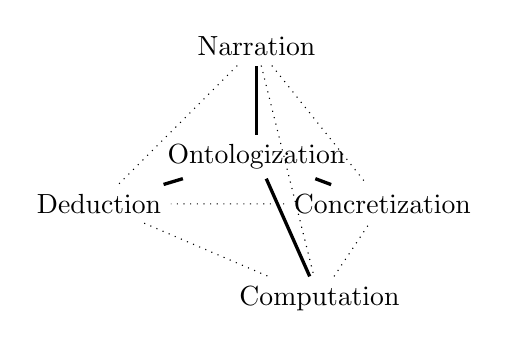
\begin{tikzpicture}[scale=4]
  \node (center) at (0,.15) {Ontologization};
  \node (left) at (.2,-.3) {Computation};
  \node (right) at (.4,0) {Concretization};
  \node (back) at (-.5,0) {Deduction};
  \node (up) at (0,.5) {Narration};

  \draw[very thick] (center) -- (left);
  \draw[very thick] (center) -- (right);
  \draw[very thick] (center) -- (back);
  \draw[very thick] (center) -- (up);
  \draw[dotted] (left) -- (right) -- (back) -- (left);
  \draw[dotted] (up) -- (left);
  \draw[dotted] (up) -- (right);
  \draw[dotted] (up) -- (back);
\end{tikzpicture}
\end{center}
\caption{Tetrapod model of knowledge}\label{fig:tetrapod}
\end{figure}

\begin{figure}[htb]\centering\footnotesize\setlength{\tabcolsep}{4pt}
\begin{tabular}{|l|llp{2.1cm}l|}\hline
       & \multicolumn{4}{c|}{characteristic} \\
Aspect &  objects & advantage & joint advantage of the other aspects & application \\\hline
deduction & formal proofs & correctness & ease of use & verification \\
computation & programs & efficiency & well-definedness & execution\\
concretization & concrete objects & tangibility & abstraction & storage/retrieval\\
narration & texts & flexibility & formal semantics & human understanding\\\hline
\end{tabular}
\quad
\begin{tabular}{|l|l|}\hline
Aspect pair & characteristic advantage \\\hline
ded./comp.  & rich meta-theory \\
narr./conc. & simple languages \\\hline
ded./narr.  & theorems and proofs \\
comp./conc. & normalization \\\hline
ded./conc.  & decidable well-definedness \\
comp./narr. & Turing completeness \\\hline
\end{tabular}
\caption{Shared properties and advantages of aspects}\label{fig:tetrapod2}
\end{figure}

Most approaches try to incorporate all or multiple aspects.
But all languages and tools tend to be heavily biased towards and optimized for a single one of the four corner aspects.
This is not due to ignorance but because each aspect provides characteristic advantages that are extremely hard to capture at once.
In fact, every combination of aspects shares characteristic advantages and disadvantages as sketched in Figure~\ref{fig:tetrapod2}.
For example, deductive and narrative definitions of a function involved well-definedness arguments, and a function defined by a concrete table is trivially well-defined, but a computational definition of a function may throw exceptions when running; but only the latter can store and compute functions efficiently.
Consequently, dedicated and mostly disjoint communities have evolved that have produced large aspect-specific datasets.

%\subsection{Aspect-Specific Datasets in Mathematics}
%
%A survey of the state of the art in aspects is huge.
%Figure~\ref{fig:libraries} gives an overview of important datasets just the domain of mathematics.
%We have also pre-published a draft of an extensive survey in \cite{CarFarSharBerKohMueRab:somss20}.
%
%Crucially, these disjoint projects overlap massively.
%For example, the concept of \emph{group} is defined in most proof assistants and computer algebra systems, concrete groups are part of multiple large libraries (e.g., as the main object of interest in the small groups libraries, or as symmetry groups arising from other objects), and has entries in most narrative libraries (e.g., with entries in Stacks and nLab).
%Despite the overwhelming practical need, at the moment there is little to no technology to integrate libraries across this overlap.
%The same effect is found in other domains.
%
%\begin{figure}[ht]\centering\small\def\cite#1{}
%  \begin{tabular}{| p{.3\textwidth} | p{0.55\textwidth}|}\hline
%  Dataset & Description and approximate size \\\hline\hline
%  \multicolumn{2}{|l|}{\textbf{Inference}} \\\hline
%  Theorem prover libraries  & ??? \\\hline
%  \multicolumn{2}{|l|}{\textbf{Computation} \hfill\strut\hfill {\tiny CAS = computer algebra system}} \\\hline
%  Mathematica & commercial CAS, $5k$ built-in functions, $150$k official examples\\\hline
%  Maple & commercial CAS, $5$k built-in functions \\\hline
%  GAP \cite{gap} & CAS for group theory, $10$k statements \\\hline
%  Singular \cite{singular:on} & CAS for polynomials, over $90$ libraries \\\hline
%  SageMath \cite{SageMath:on} & $1$k modules, bundled with $4$GB of CAS tools and libraries\\\hline
%  Modelica \cite{Modelica:on} & modeling language, $5$k built-in classes, $100$ open source libraries, $50$ commercial libraries up to $0.5$M equations \\\hline\hline % $10$ official, $>100$ open-source, $50$ commercial,
%  \multicolumn{2}{|l|}{\textbf{Concretization}} \\\hline
% OEIS \cite{OEIS:on} & $330$k integer sequences, $1$ TB; $0.3$M sequence identities in \cite{kwarc:datahost:on} \\\hline
%%  OEIS identities \cite{kwarc:datahost:on} & $0.3$M sequence identities, $2.5$ TB \\\hline
% various databases of graphs\cite{ConderCensuses:on, HartleyPolytopes:on, LeemansPolytopes:on, PotocnikCensuses:on, RoyleVT:on, WilsonET:on} & highly symmetric graphs, maps, polytopes, $30$ datasets, $2$M objects, $1$TB \\\hline
%  various databases of lattices \cite{KohLat:on, LeeLat:on, MalLat:on} & $7$ datasets, $17$G objects, $1.5$ TB \\\hline
%  findstat \cite{findstat} & combinatorial statistics and maps, $1.5$k objects \\\hline
%  SageMath databases \cite{SageDB:on} & $12$ datasets \\\hline
%  $L$-functions and modular forms \cite{lmfdb:on} & $80$ datasets, $1$G objects, $1$ TB \\\hline
%  Small Groups Library \cite{BeEiOBSmallGroups} & $450$M groups, $80$ MB \\\hline\hline
%  \multicolumn{2}{|l|}{\textbf{Narration}\hfill\strut\hfill {\tiny based on publications (P) or concepts (C)}} \\\hline
%  arXiv.org (P) & $300$k math preprints, most with {\LaTeX} sources\\\hline
%  zbMATH \cite{zbMATH:on} (P) & $4$M publication abstracts with semantic data, $30$M reference data, $1$M disambig. authors, $2.7$M full text links \\\hline % $1$M OA 
%  EuDML  \cite{EuDML:on} (P) & $260$k open full-text publications, digitized journal back issues \\\hline
%%  MathOverFlow & $\approx 1,1$M questions/answers, $\geq11$K answer authors \\\hline
%  Stacks project (C) & $6$k pages, semantically annotated, curated, searchable textbook \\\hline
%  $n$Lab (C) & $13$k pages on category theory and applications\\\hline
%  SMGloM glossary (C) & $1$k modules, $2$k concepts, $4.5$k multi-lingual verbalizations in English \\\hline\hline %  (100\%), German (90\%), Chinese (10\%)
%  \multicolumn{2}{|l|}{\textbf{Organization}} \\\hline
%  swMATH \cite{swMATH:on} & $25$k software records with $300$k links to $180$k publications \\\hline
%  Wikidata  \cite{wikidata:on} & $34$GB linked data, $4$k formulas, interlinked with named theorems, persons, publications \\\hline
%  DLMF & $500$ special mathematical functions, $10$k formulas \\\hline
%  OpenMath CDs \cite{openmath} & curated reference points for $1.5$k concepts \\\hline
%  LATIN atlas \cite{CHKMR:latinabs:11,LATIN:online} & modular definitions of logics, $1$k modules \\\hline
%  Formal Abstracts  \cite{fabstracts} & formal definitions for all concepts used by multiple authors of mathematical papers (planned) \\\hline
%  \oaf interface library & as obtained in \oaf WP 2.6\\\hline
%\end{tabular}
%  \caption{Representative examples of large libraries by aspect}\label{fig:libraries}
%\end{figure}


\chapter{Overview of This Course}
  \section{Structure}

The subsequent \emph{parts} of this course follow the Tetrapod model with one part per aspect.
Each of these will describe the concepts, languages, and tools of the respective aspect as well as their relation to other aspects.

The aspects of the Tetrapod are typically handled in individual courses, which describe highly specialized languages and tools in depth.
On the contrary, the overall goal of this course will be seeing all of them as different approaches to semantics and knowledge representation.
The course will focus on universal principles and their commonalities and differences as well as their advantages and disadvantages.

The subsequent \emph{chapters} of this first part will be dedicated to aspect-independent material.
These will not necessarily be taught in the order in which they appear in these notes.
Instead, some of them will be discussed in connection to how they are relevant in individual aspects.

\section{Exercises and Running Example}

Typical practical projects, e.g., the ones that a strong CS graduate might be put in charge of, involve heterogeneous data and knowledge that must be managed using a variety of optimized aspect-specific languages and tools.
Interoperability between these is often a major source of inefficiency and bugs.

The exercises accompanying the course will mimic this situation: they will be designed around a single large project that requires choosing and integrating methods, languages, and tools from all aspects.

Concretely, this project will be the development of a univis-like system for a university.
It will involve heterogeneous data such as course and program descriptions, legal texts, websites, grade tables, and transcript generation code.

Over the course of the semester students will implement a completely functional system applying the lessons of the course.
This is very unusual and often impossible for other courses: as any university course must teach many different things from a wide area, it is rarely possible to find a project that requires many and only lessons from a single course.
Here KRP is special because its material pervades all aspects of system development.



\chapter{Representing Syntax and Semantics}\label{sec:wuv:syntax}
%\footnote{This chapter is grouped with the general parts to whom it belongs conceptually. But in the lecture it was treated later.}
  \section{Context-Free Syntax}

Abstractly, context-free syntax is specified using grammars.
Concretely, it is implemented using inductive types.

In the sequel, we will start with the standard definitions and then make a series of variation to each of these definitions until they become equivalent.
The intended equivalence is as follows:
\begin{center}
\begin{tabular}{l|l}
CFG & IDT \\
\hline
non-terminal & type \\
production & constructor \\
non-terminal on left of production & return type of constructor \\
non-terminals on right of production & arguments types of constructor \\
terminals on right of production & notation of constructor
\end{tabular}
\end{center}

%%%%%%%%%%%%%%%%%%%%%%%%%%%%%%
\subsection{Context-Free Grammars}

We start with the usual definition:

\begin{definition}[Context-Free Grammar]
Given a set $\Sigma$ of characters (containing the terminal symbols), a \textbf{context-free grammar} consists of
\begin{compactitem}
\item a set $N$ of names called \textbf{non-terminal symbols}
\item a set of \textbf{productions} each consisting of
 \begin{compactitem}
  \item an element of $N$, called the \textbf{left-hand side}
  \item a word over $\Sigma\cup N$, called the \textbf{right-hand side}
 \end{compactitem}
\end{compactitem}
\end{definition}

\begin{example}
Let $\Sigma=\{0,1,+,\cdot,\doteq,\leq\}$.
We give a grammar for arithmetic expressions and formulas about them:
\begin{commgrammar}
\gprod{E}{0}{}\\
\galtprod{1}{}\\
\galtprod{E+E}{}\\
\galtprod{E\cdot E}{}\\
\gprod{F}{E\doteq E}{}\\
\galtprod{E\leq E}{}\\
\end{commgrammar}
Here we use the BNF style of writing grammars, where the productions are grouped by their left-hand side and written with $\bbc$ and $\bnfalt$.
We have $N=\{E,F\}$.
\end{example}

First, we give a name to each production of a CFG:

\begin{definition}[Context-Free Grammar with Named Productions]
Given a set $\Sigma$ of characters (containing the terminal symbols), a \textbf{context-free grammar} consists of
\begin{compactitem}
\item a set $N$ of names called \emph{non-terminal symbols}
\item a set of \emph{productions} each consisting of
 \begin{compactitem}
  \item a name
  \item an element of $N$, called the \textbf{left-hand side}
  \item a word over $\Sigma\cup N$, called the \textbf{right-hand side}
 \end{compactitem}
\end{compactitem}
\end{definition}

\begin{example}
The grammar from above with names written to the right of each production
\begin{commgrammar}
\gprod{E}{0}{zero}\\
\galtprod{1}{one}\\
\galtprod{E+E}{sum}\\
\galtprod{E\cdot E}{product}\\
\gprod{F}{E\doteq E}{equality}\\
\galtprod{E\leq E}{lessOrEqual}\\
\end{commgrammar}
This is not common BNF anymore.
\end{example}

Then we add base types to the productions:

\begin{definition}[Context-Free Grammar with Named Productions and Base Types]
Given a set $\Sigma$ of characters (containing the terminal symbols) and a set $T$ of names (containing the base types allowed in productions), a \textbf{context-free grammar} consists of
\begin{compactitem}
\item a set $N$ of names called \emph{non-terminal symbols}
\item a set of \emph{productions} each consisting of
 \begin{compactitem}
  \item a name
  \item an element of $N$, called the \textbf{left-hand side}
  \item a word over $\Sigma\cup T\cup N$, called the \textbf{right-hand side}
 \end{compactitem}
\end{compactitem}
\end{definition}

The intuition behind base types is that we commonly like to delegate some primitive parts of the grammar to be defined elsewhere.
A typical example are literals such as numbers $0, 1, 2,\ldots$: We could give regular expression syntax for digit-strings.
Instead, it is nicer to just assume we have a set of base types that we can use to insert an infinite set of literals into the grammar.

\begin{example}
Let $Nat$ be the type of natural numbers and let $T=\{Nat\}$.
Then we can improve the grammar from above as follows:
\begin{commgrammar}
\gprod{E}{Nat}{literal}\\
\galtprod{E+E}{sum}\\
\galtprod{E*E}{product}\\
\gprod{F}{E\doteq E}{equality}\\
\galtprod{E\leq E}{lessOrEqual}\\
\end{commgrammar}
\end{example}

%%%%%%%%%%%%%%%%%%%%%%%%%%%%%%
\subsection{Inductive Data Types}

We start with the usual definition:

\begin{definition}[Inductive Data Type]\label{def:idt}
Given a set of names $T$ (containing the types known in the current context), an \emph{inductive data type} consists of
\begin{compactitem}
 \item a name, called the \textbf{type},
 \item a set of \textbf{constructors} each consisting of
 \begin{compactitem}
  \item a name $n$
  \item a list of elements of $T\cup\{n\}$, called the \textbf{argument} types
 \end{compactitem} 
\end{compactitem}
\end{definition}

\newcommand{\cons}[2]{\mathtt{#1}\,\kw{of}\,\fold{*}{#2}}
\newcommand{\indtype}[2]{#1\,=\,\fold{\;\tb|\tb}{#2}}
\newcommand{\consnot}[3]{\mathtt{#1}\,\kw{of}\,\fold{*}{#2}\,\#\,#3}
\newcommand{\consn}[2]{\mathtt{#1}\,\#\,#2}

\begin{example}
Let $Nat$ be the type of natural numbers and $T=\{Nat\}$.
We give an inductive type for arithmetic expressions:
\[
\indtype{E}{\cons{literal}{Nat}, \cons{sum}{E,E}, \cons{product}{E,E}} \\
\]
Here we use ML-style notation for inductive data types, which separates constructors by $|$ and writes them as \texttt{name of argument-type-product}.
\end{example}

First we generalize to mutually inductive types:

\begin{definition}[Mutually Inductive Data Types]
Given a set $T$ of names (containing the types known in the current context), a family of \textbf{mutually inductive data type} consists of
\begin{compactitem}
 \item a set $N$ of names, called the \textbf{types},
 \item a set of \emph{constructors} each consisting of
 \begin{compactitem}
  \item a name
  \item an element of $N$, called the \textbf{return type}
  \item a list of elements of $N\cup T$, called the \textbf{argument} types
 \end{compactitem} 
\end{compactitem}
\end{definition}

\begin{example}
We extend the type definition from above by adding a second type for formulas.
Thus, $N=\{E,F\}$.
\[\mathll{
\indtype{E}{\cons{literal}{Nat}, \cons{sum}{E,E}, \cons{product}{E,E}} \\
\indtype{F}{\cons{equality}{E,E}, \cons{lessOrEqual}{E,E}}
}\]
\end{example}

%It may look $T$ and $\Sigma$ correspond to each other.
%But that is not true, we need to add them to each definition.

Then we add notations to the constructors:

\begin{definition}[Mutually Inductive Data Types with Notations]
Given a set $\Sigma$ of characters (containing the terminal symbols) and a set $T$ of names (containing the types known in the current context), a family of \textbf{mutually inductive data type with notations} consists of
\begin{compactitem}
 \item a set $N$ of names, called the \textbf{types},
 \item a set of \emph{constructors} each consisting of
 \begin{compactitem}
  \item a name
  \item an element of $N$, called the \textbf{return type}
  \item a list of elements of $T\cup N$, called the \textbf{argument} types
  \item a word over the alphabet $\Sigma\cup T\cup N$ containing the argument types in order and only elements from $\Sigma$ otherwise, called the \textbf{notation} of the constructor
 \end{compactitem} 
\end{compactitem}
\end{definition}

The intuition behind notations is that it can get cumbersome to write all constructor applications as $Name(arguments)$.
It is more convenient to attach a notation to  such as 

\begin{example}
We extend the type definitions from above by adding notations to each constructor.
We use the set $\Sigma=\{+,\cdot,\doteq,\leq\}$ as terminals in the notations.
\[\mathll{
\indtype{E}{\consnot{literal}{Nat}{Nat}, \consnot{sum}{E,E}{E+E}, \consnot{product}{E,E}{E\cdot E}} \\
\indtype{F}{\consnot{equality}{E,E}{E\doteq E}, \consnot{lessOrEqual}{E,E}{E\leq E}}
}\]
Here we write the constructors as \texttt{name of argument-type-product \# notation}.
It is easy to see that this has introduced redundancy: we can infer the argument types from the notation.
So we can just drop the argument types:
\[\mathll{
\indtype{E}{\consn{literal}{Nat}, \consn{sum}{E+E}, \consn{product}{E\cdot E}} \\
\indtype{F}{\consn{equality}{E\doteq E}, \consn{lessOrEqual}{E\leq E}}
}\]
\end{example}


\subsection{Merged Definition}

With the variation from above we have arrived at the following equivalence:

\begin{theorem}
Given a set $\Sigma$ of characters and a set $T$ of names, the following notions are equivalent:
\begin{compactitem}
\item a family of mutually inductive data types in the context of types $T$ with notations using characters from $\Sigma$,
\item a context-free grammar with named productions, terminal symbols from $\Sigma$, and base types $T$.
\end{compactitem}
\end{theorem}
\begin{proof}
The key idea is that
\begin{compactitem}
 \item the types and constructors of the former correspond to the non-terminals and productions of the latter
 \item for each constructor-production pair
  \begin{compactitem}
   \item the right-hand side of the latter corresponds to the notation of the former,
   \item the argument types of the former correspond to the non-terminals occurring on the right-hand side of the latter.
  \end{compactitem}
\end{compactitem}
\end{proof}

In implementations in programming languages, we often drop the notations.
Instead, those are handled, if needed, by special parsing and serialization functions.

However, in an implementation, it is often helpful to additionally give names to each argument of a production/constructor.
That yields the following definition:

\begin{definition}[Context-Free Syntax]
Given a set $\Sigma$ of characters and a set $T$ of names, a context-free syntax consists of
\begin{compactitem}
 \item a set $N$ of names, called the \textbf{non-terminals/types},
 \item a set of \emph{productions/constructors} each consisting of
 \begin{compactitem}
  \item a name
  \item an element of $N$, called the \textbf{left-hand side/return type}
  \item a sequence of objects, called the \textbf{right-hand side/arguments} which are one of the following
   \begin{compactitem}
    \item an element of $\Sigma$
    \item a pair written $(n:t)$ of a name $n$, called the \textbf{argument name}, and an element $t\in T\cup N$ called the \textbf{argument type}.
   \end{compactitem}
 \end{compactitem}
\end{compactitem}
\end{definition}

\begin{example}
Using ad hoc language to write the constructors, our example from above as a context-free syntax could look as follows:
\[\mathll{
\indtype{E}{\consn{literal}{(value:Nat)}, \consn{sum}{(left:E)+(right:E)}, \consn{product}{(left:E)\cdot (right:E)}} \\
\indtype{F}{\consn{equality}{(left:E)\doteq (right:E)}, \consn{lessOrEqual}{(left:E)\leq (right:E)}}
}\]
This uses an ad hoc 
\end{example}


\section{Implementation}

Context-free syntax can be implemented systematically in all programming languages.
But, depending on the style of the language, they make drastically different.
We give the two most important paradigms as examples.

\subsection{Functional Programming Languages}

In a function programming language, inductive data types are a primitive feature.
However, notations and named arguments are not available.
So helper functions must be used.

The basic recipe is as follows:
\begin{compactitem}
\item The types and constructors (without the notations and named arguments) are implemented as family of mutually inductive data types.
\item For each argument of each constructor, a partial projective function is defined.
\item A set of mutually recursive string rendering functions are define, one for each constructor, that implement the notations.
\end{compactitem}

\begin{example}
We define our example syntax in ML.

First the inductive types (assuming a type $Nat$ already exists in the context):
\[\mathll{
\kw{data}\, \indtype{E}{\cons{literal}{Nat}, \cons{sum}{E,E}, \cons{product}{E,E}} \\
\kw{and}\,\indtype{F}{\cons{equality}{E,E}, \cons{lessOrEqual}{E,E}}
}\]

Now the projection functions:
\[\mathll{
 \kw{fun}\; \mathtt{literal\_value}(\mathtt{literal}(v)) = SOME\; v \\
 |\tb \mathtt{literal\_value}(\_)= NONE \\
 \kw{fun}\; \mathtt{sum\_left}(\mathtt{sum}(x,\_)) = SOME\; x \\
 |\tb \mathtt{sum\_left}(\_)= NONE\\
 \kw{fun}\; \mathtt{sum\_right}(\mathtt{sum}(\_,x)) = SOME\; x \\
 |\tb \mathtt{sum\_right}(\_)= NONE
}\]
and so on for each constructor argument.

Finally, the string rendering functions (assuming a function $natToString$ already exists in the context):
\[\mathll{
 \kw{fun}\; \mathtt{E\_toString}(\mathtt{literal}(v)) = natToString\;v \\
 |\tb \mathtt{E\_toString}(\mathtt{sum}(x,y))= \mathtt{E\_toString}(x) + "+" + \mathtt{E\_toString}(y) \\
 |\tb \mathtt{E\_toString}(\mathtt{product}(x,y))= \mathtt{E\_toString}(x) + "\cdot" + \mathtt{E\_toString}(y) \\
 \kw{and}\; \mathtt{F\_toString}(\mathtt{equality}(x,y)) = \mathtt{E\_toString}(x) + "\doteq" + \mathtt{E\_toString}(y)\\
 |\tb \mathtt{F\_toString}(\mathtt{lessOrEqual}(x,y)) = \mathtt{E\_toString}(x) + "\leq" + \mathtt{E\_toString}(y)
}\]
\end{example}

Because ML has inductive data types as primitives, pattern-matching on our syntax comes for free.
We will get back to that when defining the semantics.

\subsection{Object-Oriented Programming Languages}

In a object-oriented programming language, inductive data types are not available.
Therefore, they must be mimicked using classes.
On the positive side, this supports arguments names, and notations are a bit easier.

The basic recipe is as follows:
\begin{compactitem}
\item Each types is implemented as an abstract class.
\item Each constructor of type $t$ is implemented as a concrete class that extends the abstract class $t$.
\item The arguments names and type of each constructor $c$ are exactly the argument names and types of the class $c$.
The constructor arguments are stored as fields in the class.
\item The abstract classes require a \texttt{toString} method, which is implemented in every concrete class according to its notation.
\end{compactitem}


\begin{example}
We define our example syntax in a generic OO-language somewhat similar to Scala.\footnote{We could use Java or C++ here. But their concrete syntax makes this less clear than it could be. It is straightforward to refine the syntax into that of any specific OO-language.}

In particular, we assume that the sy

\begin{lstlisting}
abstract class E {
  def toString: String
}
class literal extends E {
  field value: Nat
  constructor (value: Nat) {
    this.value = value
  }
  def toString = value.toString
}
class sum extends E {
  field left: Nat
  field right: Nat
  constructor (left: E, right: E) {
    this.left = left
    this.right = right
  }
  def toString = left.toString + "+" + right.toString
}
class product extends E {
  field left: Nat
  field right: Nat
  constructor (left: E, right: E) {
    this.left = left
    this.right = right
  }
  def toString = left.toString + "$\cdot$" + right.toString
}

abstract class F {
  def toString: String
}
class equality extends E {
  field left: Nat
  field right: Nat
  constructor (left: E, right: E) {
    this.left = left
    this.right = right
  }
  def toString = left.toString + "$\doteq$" + right.toString
}
class product extends E {
  field left: Nat
  field right: Nat
  constructor (left: E, right: E) {
    this.left = left
    this.right = right
  }
  def toString = left.toString + "$\leq$" + right.toString
}
\end{lstlisting}
\end{example}

Because OO-languages do not have inductive data types as primitives, pattern-matching on our syntax requires awkward switch statements.
We will get back to that when defining the semantics.

\subsection{Combining Paradigms}

The Scala language combines ideas from functional and OO-programming.
That makes its representation of context-free syntax particularly elegant.

In Scala, the constructor arguments are listed right after the class name.
These are automatically fields of the class, and a default constructor always exists that defines those fields.
That gets rid of a lot of boilerplate.

If we want to make those fields public (and we do because those are the projection functions, we add the keyword \texttt{val} in front of them.
But even if that is too much boilerplate. So Scala defines a convenience modifier: if we put \texttt{case} in front of the classes corresponding to constructors of our syntax, Scala puts in the \texttt{val} automatically.
It also generates a default implementation of \texttt{toString}, which we have to override if we want to implement notations, too.
Finally, Scala also generates pattern-matching functions so that we can pattern-match in the same way as in ML.

Then our example becomes (as usual, assuming a class \texttt{Nat} already exists):

\begin{lstlisting}
abstract class E {
  def toString: String
}
case class literal(value: Nat) extends E {
  override def toString = value.toString
}
case class sum(left: Nat, right: Nat) extends E {
  override def toString = left.toString + "+" + right.toString
}
case class product(left: Nat, right: Nat) extends E {
  override def toString = left.toString + "$\cdot$" + right.toString
}

abstract class F {
  def toString: String
}
case class equality(left: Nat, right: Nat) extends E {
  override def toString = left.toString + "$\doteq$" + right.toString
}
case class lessOrEqual(left: Nat, right: Nat) extends E {
  override def toString = left.toString + "$\leq$" + right.toString
}
\end{lstlisting}

\section{Semantics as a Recursive Function}

The correspondence for the syntax between context-free grammars and inductive data types can be extended to the semantics.
Now we have a correspondence between case-based function definitions and inductive functions.
%The equivalence is as follows:
%\begin{center}
%\begin{tabular}{l|l}
%syntax & case-based function & recursive function \\
%\hline
%non-terminal $N$ & function $N$ & function with input $x:N$\\ 
%production & constructor \\
%non-terminal on left of production & return type of constructor \\
%non-terminals on right of production & arguments types of constructor \\
%terminals on right of production & notation of constructor
%\end{tabular}
%\end{center}


%\section{Context-Sensitive Syntax}



\chapter{Encoding Data}\label{sec:wuv:codecs}
%\footnote{This chapter is grouped with the general parts to whom it belongs conceptually. But in the lecture it was treated after the parts on ontological and concretized knowledge, which motivate it.}
  \footnote{This chapter is grouped with the general parts to whom it belongs conceptually. But in the lecture it was treated after the parts on ontological and concretized knowledge, which motivate it.}

\section{Data Representation Languages}

\section{Typed Data}

\section{Encoding Typed Data in Untyped Representation Languages}

\part{Ontological Knowledge}\label{sec:wuv:ont}

\chapter{Ontologies}
 \section{General Principles}

\paragraph{Motivation}
An ontology is an abstract representation of the main concepts in some domain.
Here \emph{domain} refers to any area of the real world such as mathematics, biology, diseases and medications, human relationships, etc.
Many examples can be found at \url{https://bioportal.bioontology.org/}, including the Gene ontology one of the biggest.

Contrary to the other four aspects, ontological knowledge representations do not aim at capturing the entire semantics of the domain objects.
Instead, they focus on defining unique identifiers for the those objects and describing some of their properties and relations to each other.

We use the word \textbf{ontologization} to refer to the process of organizing the knowledge of a domain in ontologies.

Ontologies are most valuable when they are \emph{standardized} (either sanctioned through a formal body or a quasi-standard because everyone uses it).
A standard ontology allows everybody in the domain to use the identifiers defined by the ontology in a way that avoids misunderstandings.
Thus, in the simplest form, an ontology can be seen as a dictionary defining the technical terms of a domain.
For example, the Gene ontology defines identifier \texttt{GO:0000001} to have the formal name "mitochondrion inheritance" and the informal definition "The distribution of mitochondria, including the mitochondrial genome, into daughter cells after mitosis or meiosis, mediated by interactions between mitochondria and the cytoskeleton.".

\paragraph{Ontology Languages}
An ontology is written in \textbf{ontology language}.
Common ontology languages are
\begin{compactitem}
 \item description logics such as ALC,
 \item the W3C ontology language OWL, which is the standard ontology languages of the semantic web,
 \item the entity-relationship model, which focuses on modeling rather than formal syntax,
 \item modeling languages like UML, which is the main ontology language used in software engineering.
\end{compactitem}

Ontology languages are not committed to a particular domain --- in the Tetrapod model, they correspond to programming languages and logics, which are similarly uncommitted.
Instead, an ontology language is a formal language that standardizes the syntax of how ontologies can be written as well as their semantics.

\paragraph{Ontologies}
The details of the syntax vary between ontology languages.
But as a general rule, every \textbf{ontology} declares
\begin{compactitem}
 \item \textbf{individuals} --- concrete objects that exist in the real world, e.g., "Florian Rabe" or "WuV"
 \item \textbf{concepts} --- abstract groups of individuals, e.g., "instructor" or "course"
 \item \textbf{relations} --- binary relations between two individuals, e.g., "teaches"
 \item \textbf{properties} --- binary relations between an individuals and a concrete value (a number, a date, etc.), e.g., "has-credits"
 \item \textbf{concept assertions} --- the statement that a particular individual is an instance of a particular concept
 \item \textbf{relation assertions} --- the statement that a particular relation holds about two individuals
 \item \textbf{property assertions} --- the statement that a particular individual has a particular value for a particular property
 \item \textbf{axioms} --- statements about relations between concepts, typically in the form subconcept of statements like "instructor" $\sqsubseteq$ "person"
\end{compactitem}

All assertions can be understood and spoken as subject-predicate-object \textbf{triples} as follows:
\begin{center}
\begin{tabular}{l|lll}
Assertion & \multicolumn{3}{c}{Triple} \\
          & Subject & Predicate & Object \\
\hline
concept assertion  & "Florian Rabe" & \texttt{is-a} & "instructor" \\
relation assertion & "Florian Rabe" & "teaches" & "WuV" \\
property assertion & "Florian Rabe" & "has credits" & 7.5 \\
\end{tabular}
\end{center}
This uses a special relation \texttt{is-a} between individuals and concepts.
Some languages group \texttt{is-a} with the other binary relations between individuals for simplicity although it is technically a little different.

The possible values of properties must be fixed by the ontology language.
Typically, it includes at least standard types such as integers, floating point numbers, and strings.
But arbitrary extensions are possible such as dates, RGB-colors, lists, etc.
In advanced languages, it is possible that the ontology even introduces its own basic types and values.

Ontologies are often divided into two parts:
\begin{compactitem}
 \item The \textbf{abstract} part contains everything that holds in general independent of which individuals: concepts, relations, properties, and axioms.
 It describes the general rules how the worlds works without committing to a particular set of inhabitants of the world.
 This part is commonly called the \textbf{TBox} (T for terminological).
 \item The \textbf{concrete} part contains everything that depends on the choice of individuals: individuals and assertions.
 It populates the world with inhabitants.
 This part is commonly called the \textbf{ABox} (A for assertional).
\end{compactitem}


\paragraph{Synonyms}
Because these principles pervade all formal languages, many competing synonyms are used in different domains.
Common synonyms are:
\begin{center}
\begin{tabular}{l|llll|l}
 Here       & OWL      & Description logics & ER model & UML & semantics via logics\\
\hline
 individual & instance & individual & entity & object, instance & constant\\
 concept    & class    & concept &  entity-type & class & unary predicate\\
 relation   & object property & role & role & association & binary predicate \\
 property   & data property   & (not common) & attribute & field of base type & binary predicate\\
\end{tabular}
\end{center}

In particular, the individual-concept relation occurs everywhere and is known under many names:
\begin{center}
\begin{tabular}{l|ll}
 domain & individual & concept \\
\hline
type theory, logic & constant, term & type \\
set theory  & element & set \\
database    & row & table \\
philosophy\footnote{as in \url{https://plato.stanford.edu/entries/object/}} & object & property \\
grammar & proper noun & common noun \\
\end{tabular}
\end{center}

\section{A Basic Ontology Language}

\newcommand{\kw}[1]{\textbf{#1}}
\renewcommand{\bnf}[1]{{\color{red}#1}}
%\newcommand{\sem}[1]{\llbrack #1 \rrbrack}

\newcommand{\ID}{\texttt{ID}}
\newcommand{\dom}{\mathrm{dom}}
\newcommand{\rng}{\mathrm{rng}}
\newcommand{\itg}{\cn{int}}
\makecn{bool}
\makecn{float}
\newcommand{\strg}{\cn{string}}

\begin{figure}[hbt]
\begin{commgrammar}
\gcomment{Ontologies}\\
\gprod{O}{\rep{D}}{}\\
\gcomment{Declarations}\\
\gprod{D}{\kw{individual}\; \ID}{atomic individual}\\
\galtprod{\kw{concept}\; \ID}{atomic concept}\\
\galtprod{\kw{relation}\; \ID}{atomic relation}\\
\galtprod{\kw{property}\; \ID: T}{atomic property}\\
\galtprod{I\; \texttt{is-a}\; C}{concept assertion}\\
\galtprod{I\; R\; I}{relation assertion}\\
\galtprod{I\; P\; V}{property assertion}\\
\galtprod{F}{other axioms}\\
\gcomment{Formulas}\\
\gprod{F}{C \Equiv C}{concept equality}\\
\galtprod{C \sqsubseteq C}{concept subsumption}\\
\gcomment{Individual expressions}\\
\gprod{C}{\ID}{atomic individuals}\\
\gcomment{Concept expressions}\\
\gprod{C}{\ID}{atomic concepts}\\
\galtprod{C \sqcup C}{union of concepts}\\
\galtprod{C \sqcap C}{intersection of concepts}\\
\galtprod{\dom R}{domain of a relation}\\
\galtprod{\rng R}{range of a relation}\\
\gcomment{Relation expressions}\\
\gprod{R}{\ID}{atomic relations}\\
\galtprod{R ; R}{composition of relations}\\
\galtprod{R \cup R}{union of relations}\\
\galtprod{R \cap R}{intersection of relations}\\
\galtprod{R^*}{transitive closure of a relation}\\
\galtprod{\Delta_C}{identity relation of a concept}\\
\gcomment{Property expressions}\\
\gprod{P}{\ID}{atomic properties}\\
\gcomment{Identifiers}\\
\gprod{\ID}{\text{alphanumeric string}}{}\\
\gcomment{Basic types and values}\\
\gprod{T}{\itg \alt \float \alt \bool \alt \strg}{types}\\
\gprod{T}{\text{(omitted)}}{values}
\end{commgrammar}
\caption{Grammar of BOL}\label{fig:bol}
\end{figure}

We could study practical ontology languages like ALC or OWL now.
But those feature a lot of other details that can block the view onto the essential parts.
Therefore, we first define a basic ontology language ourselves in order to have full control over the details.

\subsection{Syntax}

\begin{definition}[Syntax of BOL]
A BOL-ontology is given by the grammar in Fig.~\ref{fig:bol}.
It is well-formed if
\begin{compactitem}
 \item no identifier is declared twice,
 \item every property assertion assigns a value of the type required by the property declaration,
 \item every reference to an atomic individual/concept/relation/property is declared as such.
\end{compactitem}
\end{definition}



The above grammar exhibits some general structure that we find throughout formal KR languages.
In particular, an ontology consists of \textbf{named declarations} of four different kinds as well as some axioms.
Each declaration clarifies which kind it is (in our case by starting with a keyword) and introduces a new identifier.
For each kind, there are complex expression.
These are anonymous and built inductively; their base cases are references to the corresponding identifiers.
Sometimes (in our case: individuals and properties), the references are the only expressions of the kind.
Sometimes (in our case: concepts and relations), there can be many productions for complex expressions.
The complex expressions are used to build axioms; in our case, these are the three kinds of assertions and other formulas.

\subsection{Semantics}

We give the semantics of BOL as an example of a semantics by translation.
We fix one language that we have already understood and define an interpretation function that maps all complex expression of the syntax into the semantic language.

For simple ontology languages like BOL, ALC, OWL, etc., it is common to use first-order logic (FOL) as the semantic language.
More specifically, we use SFOL, the typed variant of FOL with
\begin{definition}[Semantic of BOL]
Every BOL-ontology $O$ is interpreted as a FOL-theory $\sem{O}$ according to Fig.~\ref{fig:bolsem} where we assume that $\sem{O}$ contains
\begin{compactitem}
 \item a type $\iota$ (for individuals),
 \item additional types and constants corresponding to base types and values of BOL.
\end{compactitem}
\end{definition}

Like with the syntax, we can observe some general principles.
Every BOL-declaration is translated to a FOL declaration for the same name, and ontologies are translated declaration-wise.
For every kind of complex expression, there is one inductive function mapping BOL-expressions to FOL-expressions.
The base cases of references to declared identifiers are translated to themselves, i.e., to the identifiers of the same name declared in the FOL theory.

\begin{figure}
\begin{center}
\begin{tabular}{l|l}
BOL Syntax $X$ & Semantics $\sem{X}$ in FOL\\
\hline
\hline
ontology & FOL theory \\
$D_1,\ldots,D_n$ & $\sem{D_1},\ldots,\sem{D_n}$ \\
\hline
BOL declaration & FOL declaration \\
\kw{individual}\,$i$ & nullary function symbol $i:\iota$ \\
\kw{concept}\,$i$  & unary predicate symbol $i\sq\iota$ \\
\kw{relation}\,$i$ & binary predicate symbol $i\sq\iota\times \iota$ \\
\kw{property}\,$i:T$ & binary predicate symbol $i\sq\iota\times T$ \\
$I\; \texttt{is-a}\; C$ & axiom $\sem{C}(\sem{I})$\\
$I_1\; R\; I_2$ & axiom $\sem{R}(\sem{I_1},\sem{I_2})$\\
$I\; P\; V$ & axiom $\sem{P}(\sem{I},\sem{V})$\\
$F$ & axiom $\sem{F}$\\
\hline
Formula & Formula\\
$C_1 \Equiv C_2$ & $\forall x:\iota.\sem{C_1}(x)\Leftrightarrow \sem{C_2}(x)$\\
$C_1 \sqsubseteq C_2$ & $\forall x:\iota.\sem{C_1}(x)\impl \sem{C_2}(x)$\\
\hline
Individual & Terms of type $\iota$ \\
$i$ & $i$ \\
\hline
Concept & Formula with free variable $x:\iota$\\
$i$ & $i(x)$\\
$C_1 \sqcup C_2$ & $\sem{C_1}(x)\vee\sem{C_2}(x)$\\
$C_1 \sqcap C_2$ & $\sem{C_1}(x)\wedge\sem{C_2}(x)$\\
$\dom R$ & $\exists y:\iota.\sem{R}(x,y)$\\
$\rng R$ & $\exists y:\iota.\sem{R}(y,x)$\\
\hline
Relation & Formula with free variables $x:\iota,y:\iota$\\
$i$ & $i(x,y)$\\
$R_1 ; R_2$ & $\exists m:\iota.\sem{R_1}(x,m)\wedge \sem{R_2}(m,y)$\\
$R_1 \cup R_2$ & $\sem{R_1}(x,y)\vee \sem{R_2}(x,y)$\\
$R_1 \cap R_2$ & $\sem{R_1}(x,y)\wedge \sem{R_2}(x,y)$\\
$R^*$          & (tricky, omitted)\\
$\Delta_C$     & $x\doteq y\wedge \sem{C}(x)$\\
\hline
Property of type $T$ & Formula with free variables $x:\iota,y:T$\\
$i$ & $i(x,y)$\\
\end{tabular}
\caption{Interpretation Function for BOL}\label{fig:bolsem}
\end{center}
\end{figure}


\part{Concretized Knowledge}\label{sec:wuv:concr}

\part{Computational Knowledge}\label{sec:wuv:comp}

\part{Deductive Knowledge}\label{sec:wuv:ded}

Various methods have been developed to represent and perform inferences.
We structure our presentation by how each method relates to computation, the aspect most whose integration with inference has drawn the most attention.
In general, the ubiquity of underspecified function symbols and quantified variables means that logical expressions usually do not normalize to unique values.
At best, computations like $y:=f(x)$ can be represented as open-ended conjectures where different options for $y$ are produced, each together with a proof of the respective equality.
Therefore, inference systems usually sacrifice computation or at least its efficiency.

\emph{Proof assistants} sit at the extreme end of this spectrum.
They employ strong logics and high-level declarations to provide a convenient way to formalize domain knowledge and reason about it.
The reasoning is usually interactive in order to represent inferences that are too difficult to be fully automated.
Most proof assistants integrate at least some of the other methods to overcome this weakness.

Further along the spectrum, \emph{automated theorem provers} use simpler logics than interactive proof assistants.
They are fully automatic and much faster, but can handle much fewer theorems, and typically do not check their proofs.
\emph{Satisfiability checkers} continue this progression by aiming at decidable automation support, whereas theorem proving is usually an semi-decidable search problem.
That limits them to propositional logic or specific theories of more expressive logics (usually of first-order logic) that are complete, i.e., where every formula can be proved or disproved.
In the special cases, where satisfiability checkers are applicable, they come close to verified computation systems.

Orthogonal to the above triplet, there are several methods for realizing Turing-complete computation naturally inside a logic.
Here imperative and object-oriented computation are usually avoided in favor of other programming paradigms that are easier to reason about.
\emph{Rewriting} aims at optimizing the $f(x)\rewrites y$ progression, allowing users to mark specific transformations as rewrite steps.
\emph{Terminating recursion} is the method of adding recursive functions to a logic in order to make it a pure functional programming language.
Finally, \emph{logic programming} restricts attention to theorems of a special form, for which proof search is simple and predictable so that users can represent computations by supplying axioms that guide the proof search.


\part{Narrative Knowledge}\label{sec:wuv:narr}

\part{Conclusion}\label{sec:wuv:conc}

%\part{Appendix}
%
%\appendix
%
%\chapter{Mathematical Preliminaries}\label{sec:math}
%
\section{Power Sets}\label{sec:math:powerset}

\input{\currfiledir powerset}

\section{Relations and Functions}\label{sec:math:relfun}

\input{\currfiledir relfun}

\section{Binary Relations on a Set}\label{sec:math:binrel}

\input{\currfiledir binrel}

\section{Binary Functions on a Set}\label{sec:math:binop}

\input{\currfiledir binop}

\section{The Integer Numbers}\label{sec:math:int}

\input{\currfiledir integers}

\section{Size of Sets}\label{sec:math:setsize}

\input{\currfiledir setsize}

\section{Important Sets and Functions}\label{sec:math:sets}

\input{\currfiledir sets}

%
%\tocentryBib
%
%\input{\currfilebase.bblp}
\bibliographystyle{alpha}
\bibliography{../../../../../frabe/Program_Data/Latex/bib/rabe,../../../../../frabe/Program_Data/Latex/bib/historical,../../../../../frabe/Program_Data/Latex/bib/pub_rabe,}
%\bibliography{../../../../../homedir/Program_Data/Latex/bib/rabe,../../../../../homedir/Program_Data/Latex/bib/historical}

\end{document}